\section{Context}\label{sec:context}
In section \ref{sec:pipeline_steps}, the several steps of the data clump pipeline are outlined. However, these steps do not include how the information generated by each step is stored and how successive steps might use this information.

Therefore, a concept to store intermediate information needs to be developed. Such information might be called \textbf{context}.


Section \ref{sec:context_structure} gives a broad overview of how the context is implemented.

The serialization of the context which is important to persist the data of the several steps is then outlined in section \ref{sec:context_serialize}.

Finally, the most important context data types used by the tool are discussed in section \ref{sec:context_steps}.

\subsection{Context structure}\label{sec:context_structure}
The context is a  dynamic repository filled throughout the data clump refactoring pipeline. The context can be represented as a linked list. Each node of the list encapsulates a distinct segment of the context which is an extension of the previous context. In the beginning, there is no context and the code obtaining context is created.

When a handler needs to access information from a specific context, it needs to traverse the linked list until it finds the needed information. 


Each step in the data clump refactoring pipeline can access the context and obtain such information as it may deem necessary for its use. A step may or may not update the context. For instance, if a service performs multiple steps consecutively, it does not need to share  some information, or this would be harder to implement. To give a more concrete example, if a service can find data clumps and refactor them automatically, it might not be able to store the locations of each data clump so that respective context cannot be created. Also, a handler can create multiple chained contexts if it is capable of executing multiple steps. 




Figure \ref{fig:context_pipeline} illustrates how a different combination of handlers can affect the state of the context. The figure depicts three state diagrams where rectangles visualize the most recent context and arrows indicate executed steps.  In figure \ref{fig:context_pipeline1}, the \ac{LLM} performs the detection of data clumps, and the refactoring (including all associated sub-tasks). Because all these tasks are performed by the same service, it would be unnecessary to save intermediate results. Therefore, the context is only updated once at the conclusion of the program. This final context does not have additional information but marks that the pipeline has been executed successfully.
 

\begin{figure}[H]
\centering
  \begin{adjustbox}{minipage=\linewidth,scale=0.7}
     \centering
     \begin{subfigure}[b]{0.3\textwidth}
         \centering
         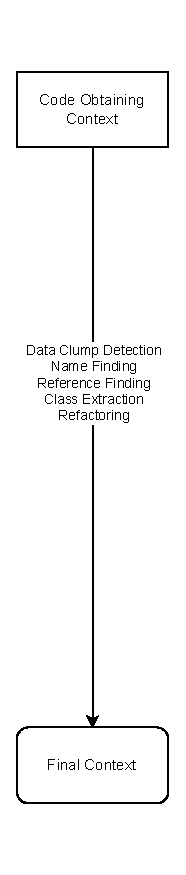
\includegraphics[width=\textwidth]{figures/chapter3/context_pipeline_1.drawio.pdf}
         \caption{All steps are performed by an \ac{LLM}}
        \label{fig:context_pipeline1}
     \end{subfigure}
     \hfill
     \begin{subfigure}[b]{0.30\textwidth}
         \centering
         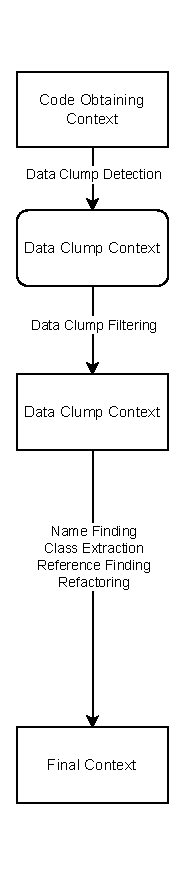
\includegraphics[width=\textwidth]{figures/chapter3/context_pipeline_2.drawio.pdf}
         \caption{Detection and filtering by another tool}
         \label{fig:context_pipeline2}
     \end{subfigure}
     \hfill
     \begin{subfigure}[b]{0.3\textwidth}
         \centering
         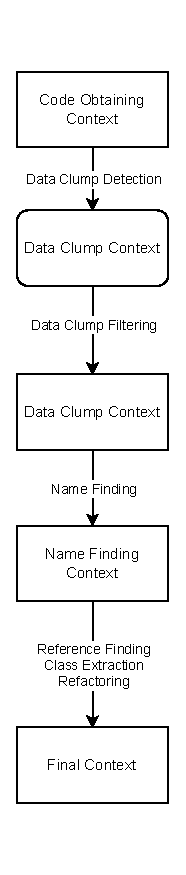
\includegraphics[width=\textwidth]{figures/chapter3/context_pipeline_3.drawio.pdf}
 \caption{Only name suggestion by an \ac{LLM}}         \label{fig:context_pipeline3}
     \end{subfigure}
        \caption{Exemplary lifecycles of the context}
        \label{fig:context_pipeline}
        \end{adjustbox}
\end{figure}

In figure \ref{fig:context_pipeline2}, some parts of the pipeline are performed by the \textit{DataClumpDoctor} and other programs. For instance, data clumps are detected by the \textit{DataClumpDoctor}. As a result, a data clump detector context is created containing all detected data clumps. Afterwards, a filter removes non-important data clump and creates a new context of the same type that is linked to the previous context. If a later handler requires information about the detected data clumps, it needs to find the first context that contains this information  beginning at the tail of the linked list. In this case it would be the filtered data clump context, not the original data clump context. Here, also the context is not updated after the filtering process as the rest of the work is performed by an \ac{LLM}. 

In figure \ref{fig:context_pipeline3}, the context is extended by a name finding context. This context includes information about a suitable identifier suggested by a \ac{LLM}. A manual refactoring tool (e.~g. IntelliJ), can use this context to perform the refactoring without further input by an \ac{LLM} so that the role of the model is limited here. 




To check whether a given pipeline is indeed executable, each step handler must describe how the context is updated when the step is executed. Each step can also specify whether a specific type of context must exist. For instance, a step may require that the \ac{AST} is available for a given source code file. 


\subsection{Context serialization}\label{sec:context_serialize}

One advantage of developing a shared context is that it can be serialized  and de-serialized with less effort. At every step of the pipeline, the current context can be  serialized into a specific location. If for some reason, the pipeline could not be executed successfully or the user of the tool is not satisfied with the result, the program does not have to be re-run, but previous results can be re-used. This is particular important in the case of persistent handlers like the \textit{DataClumpDoctor}. Re-running this service multiple times under the same parameters would have no advantage but consume resources and time. By serializing the data clump detection results, the data can be retrieved again without executing the tool again.

Another benefit of serialization is that the context can be transmitted to services easily. For instance, the service can be given the path of the serialized context which it can load. This eases communication with service  but requires that the service can understand the serialized context. 

Also, for \ac{LLM}-related steps this can be useful because every call to an \ac{LLM} induces costs. On the other hand, however, the creativity and randomness of such models can be an argument not to de-serialize such results but re-generate them so that multiple proposals can be created.



In the end, the issue of whether to use context serialization or not should depend on the service and also should be configurable by the user of the tool. 

\subsection{Context information per step}
\label{sec:context_steps}
\begin{comment}
In the following, the context created or updated after each step will be explained:

\subsubsection{Code obtaining}
The context after obtaining the source code of the project to analyze is usually the path to the project after it. In most cases, the project is defined in such a manner that there is a single base directory under which all files and directories of the project are located.

Alternatively, one could store the list of all relevant file paths of the project. This requires more storage but makes it easier to filter out files. 

\subsubsection{File Filtering}
Developing a filtering context is more challenging. One major issue is that services suitable for data clump detection offer varying solutions for including and excluding specific files. For instance, PMD which is used by the \textit{DataClumpDoctor} requires that a rule set file is located at a specific location. This rule set file contains inclusion and exclusion rules using regular expressions. 

If files are sent to an \ac{LLM}, the filtering can be performed directly on the handler level, so that more sophisticated  filtering rules can be applied without being restricted to use regular expressions. 

Because the pipeline design separates the context from the handlers, the context has limited information about the handlers and does not know which handler will be executed later. Therefore, the filtering context must be very general to maximize compatibility with all possible handlers. 

Therefore, as a design decision, the file filtering context contain only file inclusion and exclusion rules that can be applied by subsequent handlers. This means that a more complex filtering rule (e.~g. by commit date), must be resolved to a list of files to be included and excluded. 

It should also be noted that inclusion and exclusion rules might conflict, and these conflicts can be handled differently. In the case of PMD, if a file is included and excluded according to the rules, the inclusion prevails so that it is included. This makes it easier to only include a limited set of files and exclude a large number of other files. Vice versa, it is more challenging to exclude a very limited amount of files while including more files. The file filtering context does not attempt to resolve these issues. 


\subsubsection{Data clump detection and filtering}

The format described in appendix \ref{sec:data_clump_format} can be used to store the detected data clump. While this format is relatively new, it contains all relevant information for storing data clump information and is extendable. The same format can be used for filtering too as all irrelevant data clumps can be removed easily. As a result, this context is an example of a context that might appear multiple times in the linked list. 

\subsubsection{Name finding}
To store the determined names per found data clump, a dictionary can be used that maps the types-names-identifier of the data clump to a name.

One possible extension for this context could be to store multiple name suggestions for a given data clump. However, this is not part of the modeled pipeline as the benefits do not outweigh the increased complexity.

\subsubsection{Class path choosing}

At the class extraction step, the created class must be saved somewhere to be considered part of the project. The exact location can significantly impact the readability of the source code, as the location of files in a software project can help in understanding the project. 

For instance, the class could be where the data clump is initially found. This can lead to arbitrariness as the exact order of where and when data clumps are detected might not be predetermined. It should also be noted that there are always at least two parts of a data clump (e.g. two methods). As a result, if the two parts are located in separate directories, it is difficult to determine where the extracted class should be located. 

Alternatively, specific locations can be used to store all extracted classes. This, however, can also hinder readability as the extracted classes have no connections to the places where they are used. 

As an alternative, the complete class body could be stored instead of saving it directly to a file. This might be advantageous if the class content should be formatted, refactored or otherwise modified in order to be valid. This also would deflect the responsibility of the class location from the class extractor step. 

For this master thesis, the first approach is used. The type-name--key is mapped to a specific path which is chosen at the name suggestion step although it could also be chosen at the class extraction step. 

 
\subsubsection{Validation}

The validation step context requires at least information about whether the validation is successful (i.~e. no compiler errors occur and all unit tests pass). 

In case of a failed validation, one might need more information. For instance, it is helpful to know which unit test fails or on which line the code fails to compile. In many cases, modern build tools like \textit{Gradle} already acquire these data so they can be easily obtained. These error information can then be used to correct errors. 


\end{comment}

\begin{table}[ht!]
    \centering
    \begin{tabular}{m{3cm}|m{2cm}|m{5cm}|m{2cm}}
        Name & Generated in step & Contained data/methods & Serializable?  \\\hline
        Code obtaining & "" & Path to project & No \\\hline
        Git repository & Code Obtaining & Timestamps of changes in files, recently changed files & No \\\hline
        File filtering & "" & Include, exclude expression, flag for inclusion prevailment & No \\\hline

        AST & "" & \ac{AST} for each analyzed file &  Yes \\\hline
         Data clump detection & Data clump detection/filtering  & Format described in appendix \ref{app:data_clump_format}, generation of types-names-keys & Yes \\\hline 
         Name finding & "" & Names for each types-names-key & Yes\\\hline

         Class path & Name finding & Class paths for each types-names-key & Yes\\\hline

         Usage finding & "" & For each data clump: type of usage and  location & Yes \\\hline

         Validation & "" & Building successful?, error information & No \\\hline
         
    \end{tabular}
    \caption{Most important context types}
    \label{tab:context_types}
\end{table}

Table \ref{tab:context_types} shows the main context types that are created and used until the pipeline finishes. It shows the pipeline step in which the context is usually created, the operation and data it contains, and whether the context can be serialized (and hence deserialized). Quotes (") in the second column indicates that the name of the step and of the context is identical. 

One can observe that there is no one-to-one mapping between context and pipeline step. For instance, the code obtaining step generates the code obtaining context and also the Git repository context because this information is already available at this step. In other cases, two steps are using the same context. For example, the data clump detection and filtering step use the same context.

Also, the available operations differ between  the several context types. Most context types only contain the data that is initialized upon creating the respective type. In other cases, however, the context type only provides access to operations that query the sought data. For instance, the Git repository context does not load all relevant information immediately but only after it is requested. This saves performance because this information is not always used. 

Regarding serializability, it can be seen that not all context types support serialization. Only if a context contains a significant amount of data (e.~g. data clumps, usage information etc), it useful to serialize these results to save these results for further launches. 
